\label{Basic Linux network}
\chapter{Basic Linux network administration}
In this section we are going to set up a small emulated LAN of the topology in figure \ref{fig:3.1} using basic Linux network functionality and Kathará.
\begin{figure}[H]
\centering
  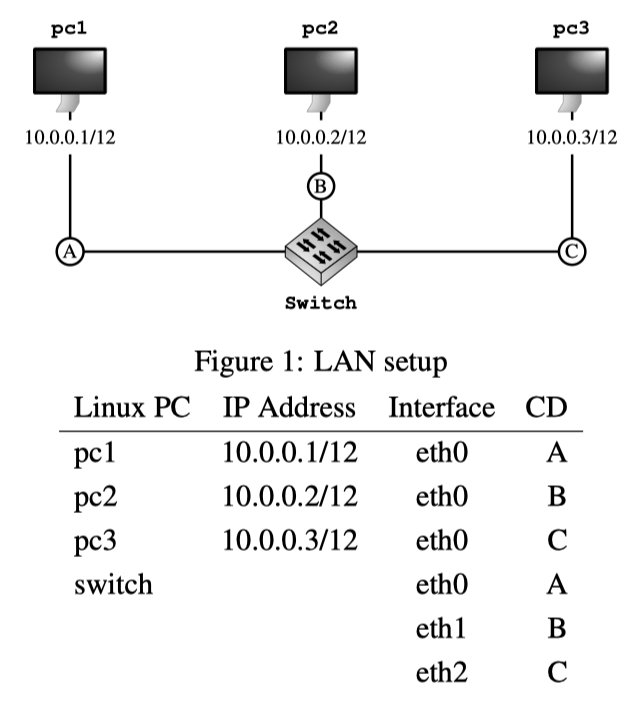
\includegraphics[width=200pt]{Images/networkFig.png}
  \caption{LAN switching configuration}
  \label{fig:3.1}
\end{figure}

\section{Creating the four devices}
\subsection{Creating Three PCs each assigned a network interface and unique collision domain}
\begin{figure}[H]
\centering
  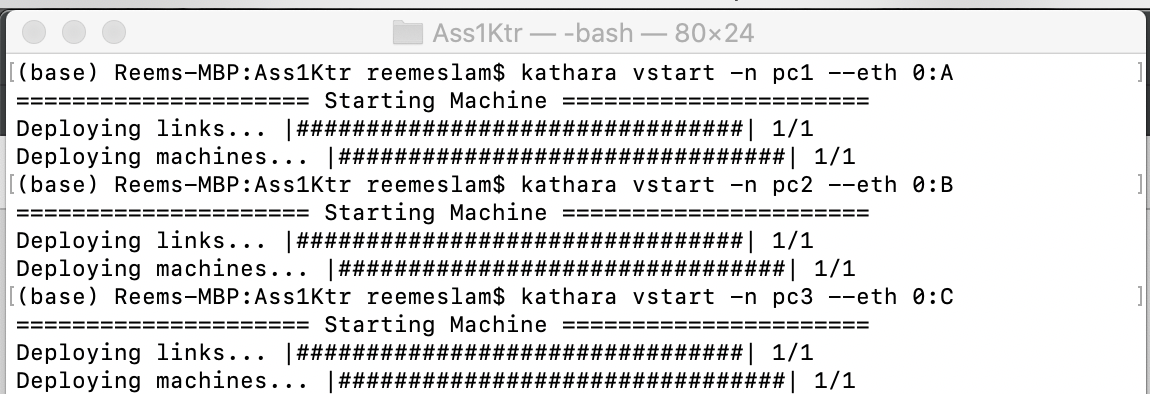
\includegraphics[width=500pt]{Images/task5.1.png}
  \caption{Created three PCs each assigned a network interface with unique collision domain}
  \label{fig:3.2}
\end{figure}

\subsection{Creating a switch that has three network interfaces attached, where each interface is connected to a different collision domain}

\begin{figure}[H]
\centering
  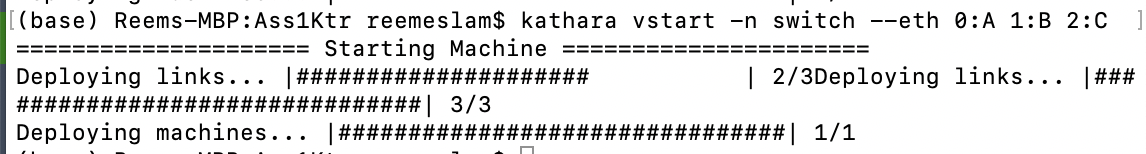
\includegraphics[width=400pt]{Images/task5.1.2.png}
  \caption{Created a Switch with three network interfaces, where each interface is connected to a different collision domain}
  \label{fig:3.3}
\end{figure}

\section{Configuring the four devices}

\subsection{Configuring an IP address for PC1, PC2 and PC2}
 \begin{figure}[H]
\centering
  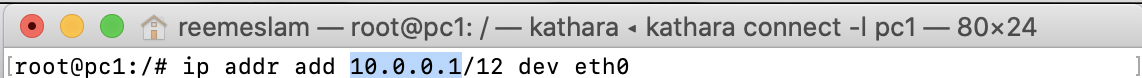
\includegraphics[width=500pt]{Images/task5.2.11.png}
  \caption{configured IP address for PC1}
  \label{fig:3.4}
\end{figure}
\begin{figure}[H]
\centering
  
\includegraphics[width=500pt]{Images/task5.2.12.png}
  \caption{configured IP address for PC2}
  \label{fig:3.5}
\end{figure}
\begin{figure}[H]
\centering
  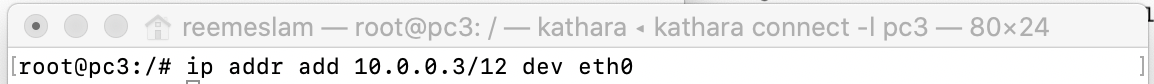
\includegraphics[width=500pt]{Images/task5.2.13.png}
  \caption{configured IP address for PC3}
  \label{fig:3.6}
\end{figure}

\subsection{Configuring a bridge for the switch, set-up the environment and turning on the bridge}

\begin{figure}[H]
\centering
  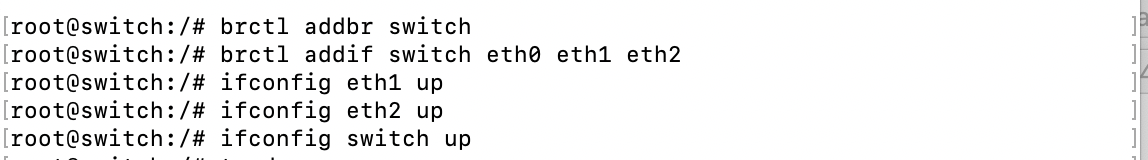
\includegraphics[width=500pt]{Images/Task5.3.png}
  \caption{Created a bridge with name switch, Added the three interfaces to the switch, turned on eth1 \& eth2 and Turned the bridge on}
  \label{fig:3.7}
\end{figure}

\subsection{Testing the network by sending pings between PCs}

\begin{figure}[H]
\centering
  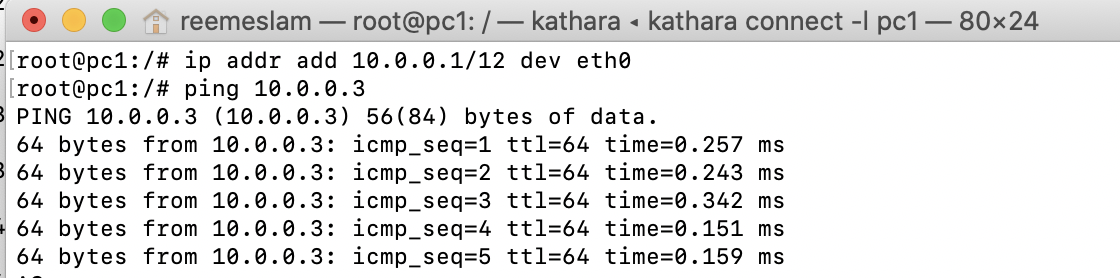
\includegraphics[width=500pt]{Images/Task5.4.1.png}
  \caption{Sending ping from PC-1 to PC-3 to check connectivity}
  \label{fig:3.8}
\end{figure}

\begin{figure}[H]
\centering
  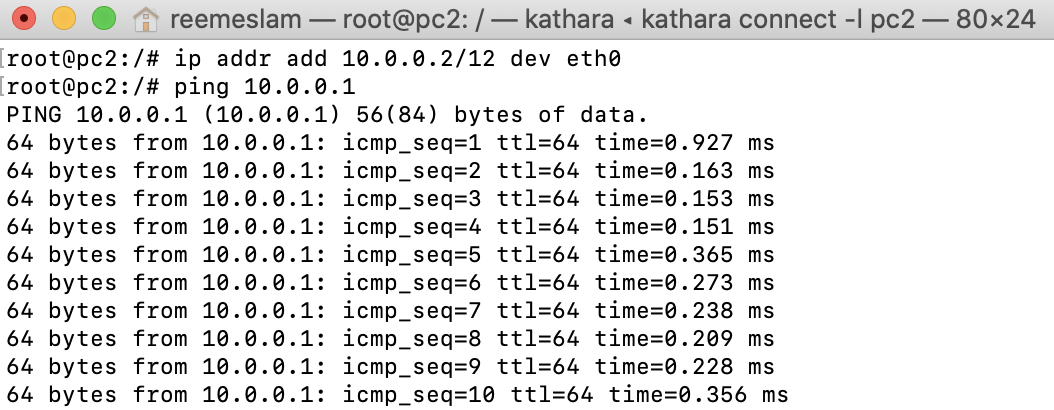
\includegraphics[width=400pt]{Images/task5.4.2.png}
  \caption{Sending ping from PC-2 to PC-1 to check connectivity}
  \label{fig:3.9}
\end{figure}

\begin{figure}[H]
\centering
  \includegraphics[width=500pt]{Images/task5.4.3.png}
  \caption{Sending ping from PC-3 to PC-2 to check connectivity}
  \label{fig:3.10}
\end{figure}

\section{Checking connectivity by Capturing the ICMP messages exchanged by devices on sending ping from Pc-1 to PC-3.}


\begin{figure}[H]
\centering
  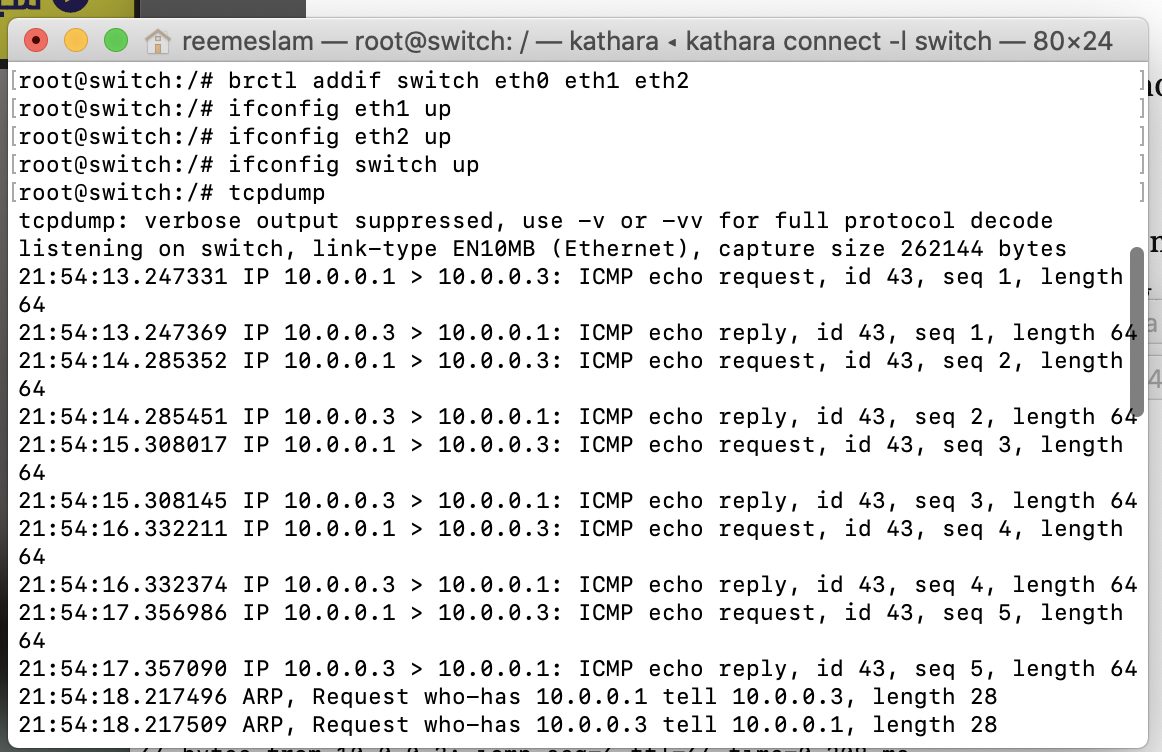
\includegraphics[width=300pt]{Images/task5.last.png}
  \caption{Capturing the ICMP messages between PC-1 and PC-3}
  \label{fig:3.11}
\end{figure}

\section{.Conf and .startup files}
For bigger complex networks using just terminals will not be the best approach, also each time you want to re-run the network you will need to configure everything again in the terminal. Better approach is to configure the environment in files and then run this files in the terminal. 
\subsection{.Conf file}
The lab.conf will help us to setup the base infrastructure when the lab is initialized. The syntax is direct and easy as we can see in \ref{fig:3.12}

\begin{figure}[H]
\centering
  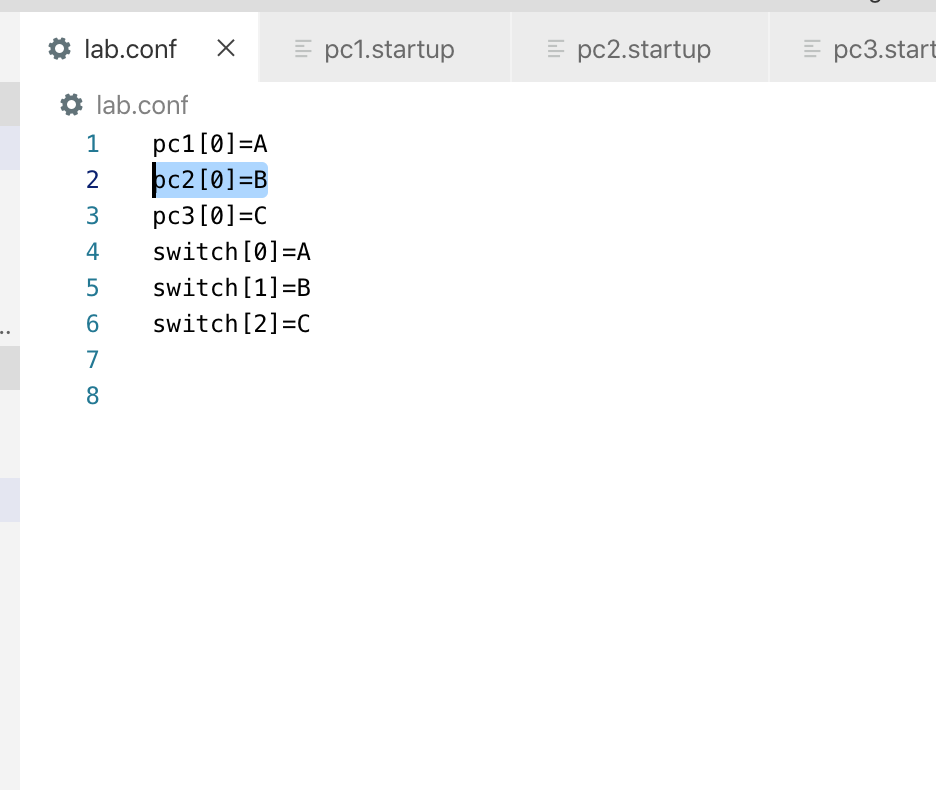
\includegraphics[width=200pt]{Images/config.png}
  \caption{The .Conf file for the network}
  \label{fig:3.12}
\end{figure}
 
\subsection{.Startup}
In .startup file we add all of the commands we want to run in each device like, configuring IP address, configuring the bridge in switch.. etc. As you can see in \ref{fig:3.13} the commands are the same as we used in the terminal.

\begin{figure}[H]
\centering
  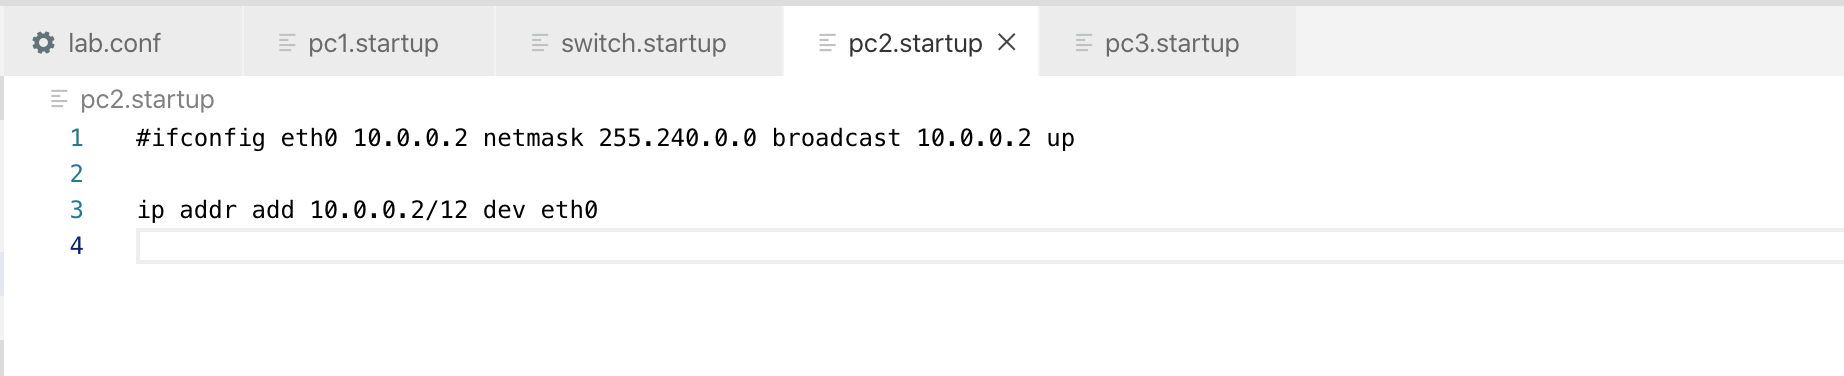
\includegraphics[width=300pt]{Images/pc2Startup.png}
  \caption{.Startup file for  PC-2 device}
  \label{fig:3.13}
\end{figure}

\begin{figure}[H]
\centering
  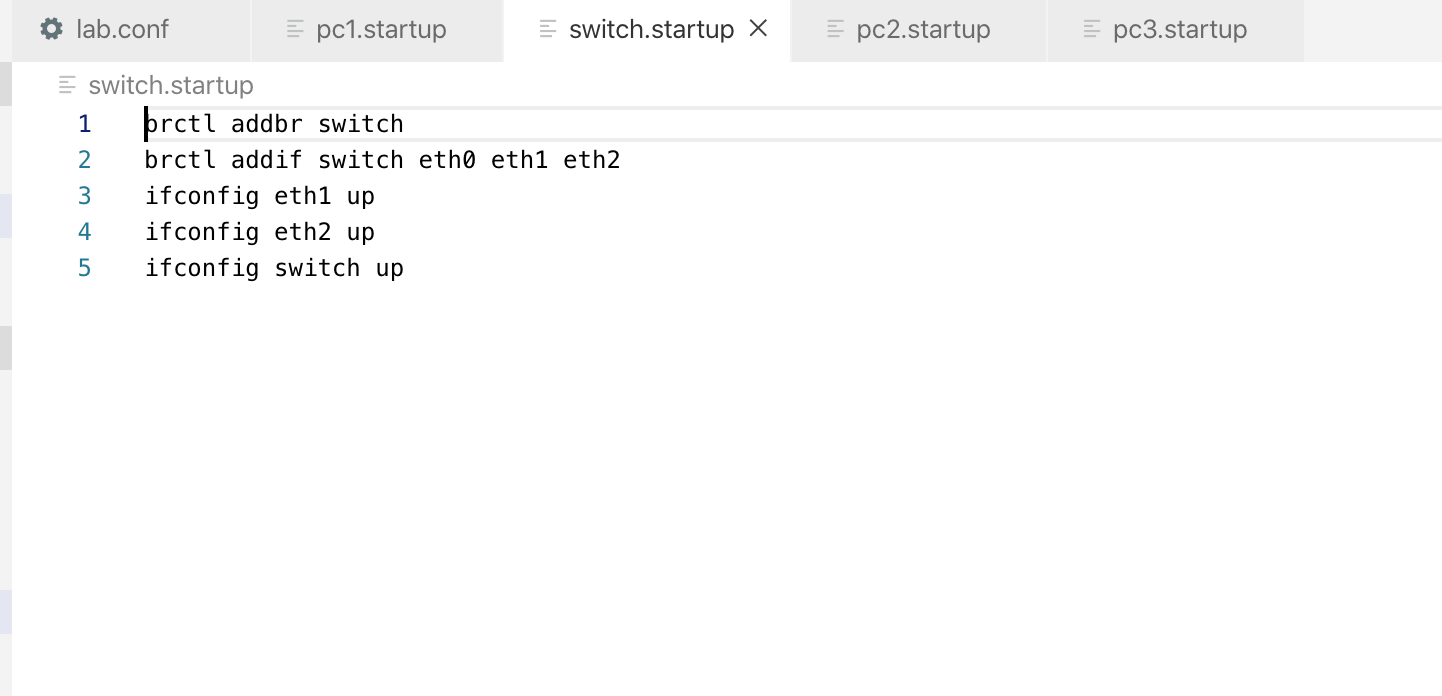
\includegraphics[width=200pt]{Images/switchstartup.png}
  \caption{.Startup file for Switch device}
  \label{fig:3.14}
\end{figure}

\clearpage
\paragraph{} 
After saving the files open the terminal in the same directory that has the files and run "Kathara lstart", The devices will open. Start testing the network by sending pings and capturing ICMP messages.

\begin{figure}[H]
\centering
  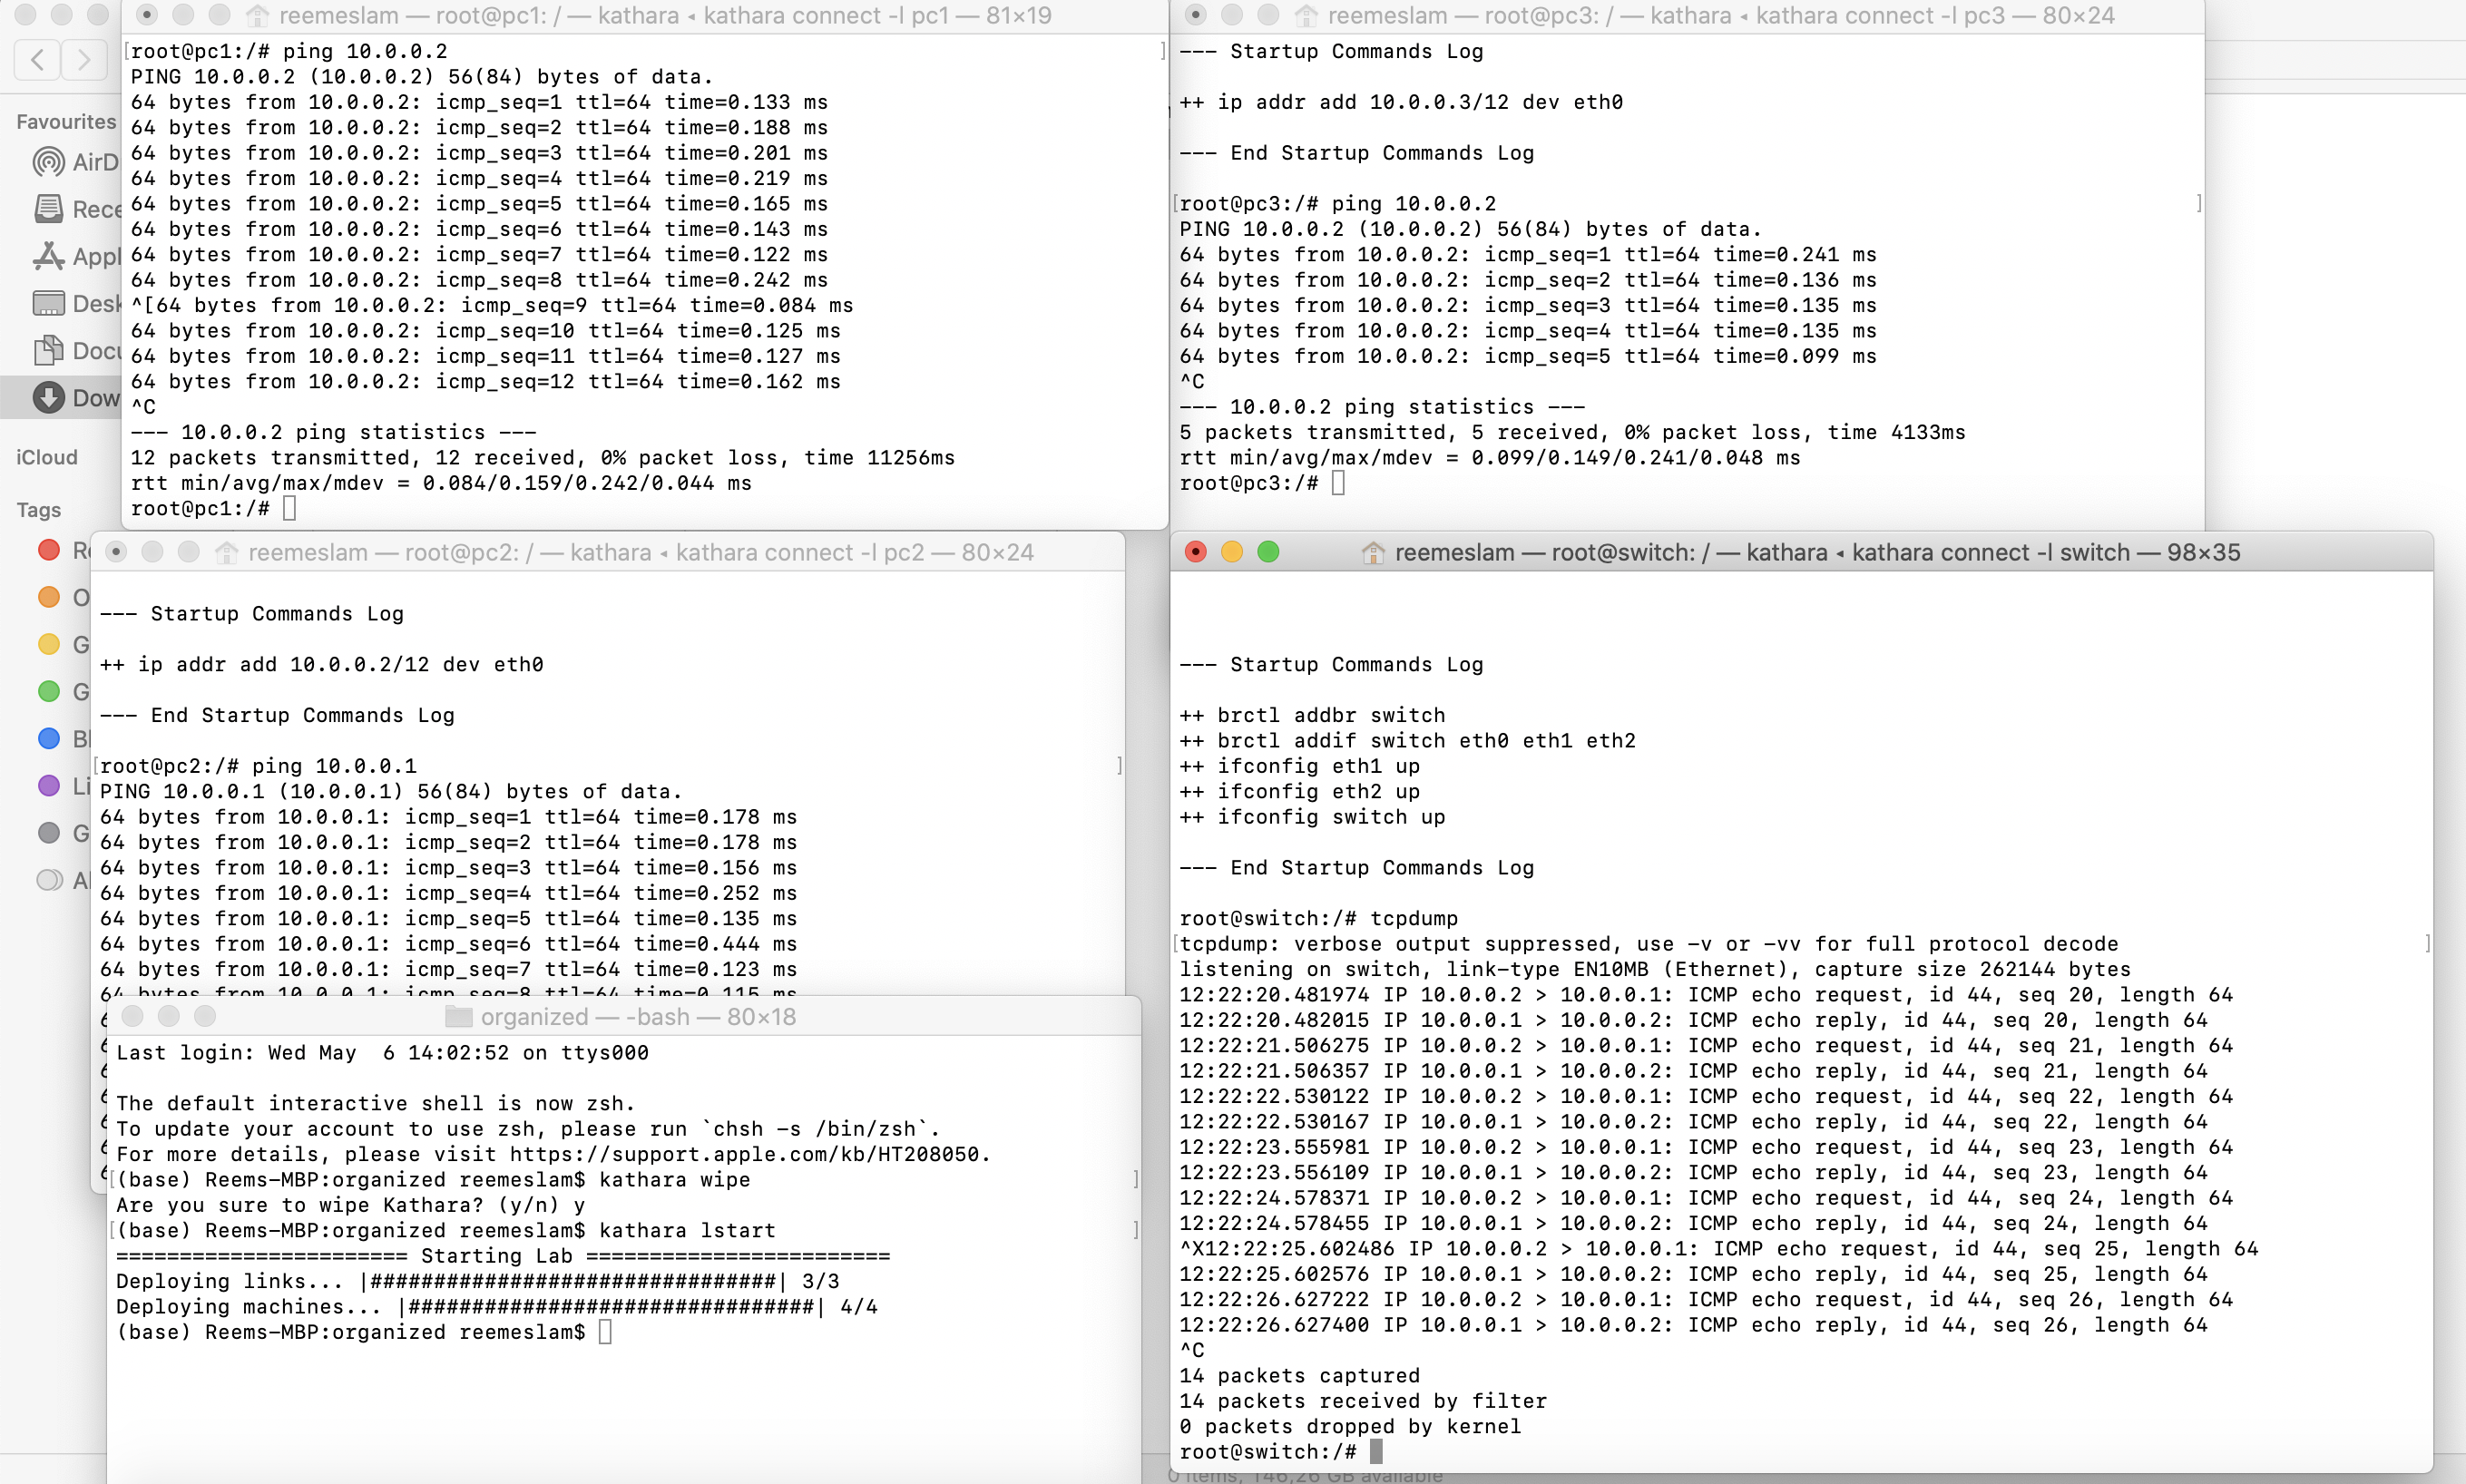
\includegraphics[width=500pt]{Images/last.png}
  \caption{Overview for the whole network}
  \label{fig:3.15}
\end{figure}